% Title: gl2ps_renderer figure
% Creator: GL2PS 1.4.0, (C) 1999-2017 C. Geuzaine
% For: Octave
% CreationDate: Mon Apr 26 23:22:59 2021
\setlength{\unitlength}{1pt}
\begin{picture}(0,0)
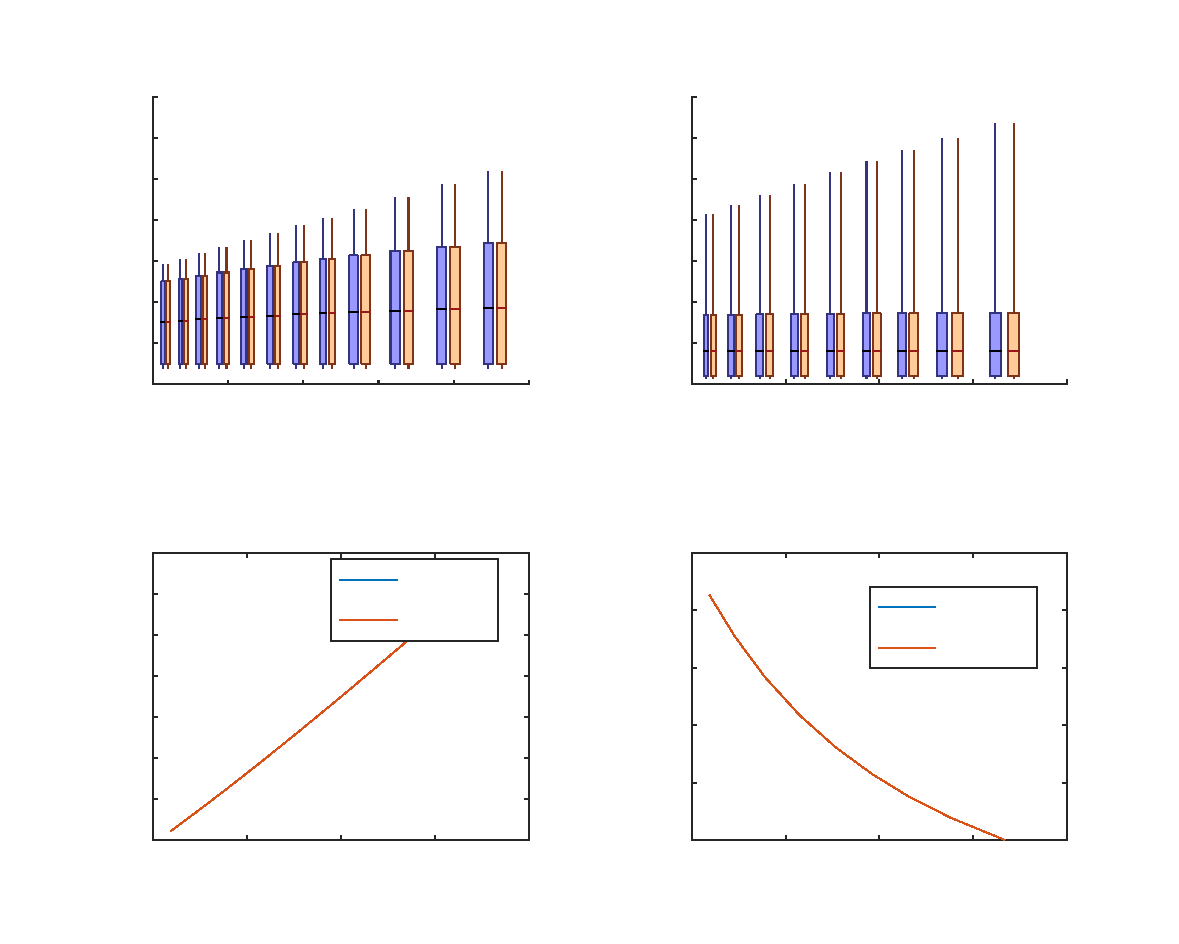
\includegraphics{FisherInformation-inc}
\end{picture}%
\begin{picture}(566,453)(0,0)
\fontsize{10}{0}
\selectfont\put(73.5801,261.175){\makebox(0,0)[t]{\textcolor[rgb]{0.15,0.15,0.15}{{0.5}}}}
\fontsize{10}{0}
\selectfont\put(109.612,261.175){\makebox(0,0)[t]{\textcolor[rgb]{0.15,0.15,0.15}{{0.6}}}}
\fontsize{10}{0}
\selectfont\put(145.644,261.175){\makebox(0,0)[t]{\textcolor[rgb]{0.15,0.15,0.15}{{0.7}}}}
\fontsize{10}{0}
\selectfont\put(181.676,261.175){\makebox(0,0)[t]{\textcolor[rgb]{0.15,0.15,0.15}{{0.8}}}}
\fontsize{10}{0}
\selectfont\put(217.708,261.175){\makebox(0,0)[t]{\textcolor[rgb]{0.15,0.15,0.15}{{0.9}}}}
\fontsize{10}{0}
\selectfont\put(253.739,261.175){\makebox(0,0)[t]{\textcolor[rgb]{0.15,0.15,0.15}{{1}}}}
\fontsize{10}{0}
\selectfont\put(68.5757,268.672){\makebox(0,0)[r]{\textcolor[rgb]{0.15,0.15,0.15}{{0}}}}
\fontsize{10}{0}
\selectfont\put(68.5757,288.379){\makebox(0,0)[r]{\textcolor[rgb]{0.15,0.15,0.15}{{0.2}}}}
\fontsize{10}{0}
\selectfont\put(68.5757,308.086){\makebox(0,0)[r]{\textcolor[rgb]{0.15,0.15,0.15}{{0.4}}}}
\fontsize{10}{0}
\selectfont\put(68.5757,327.793){\makebox(0,0)[r]{\textcolor[rgb]{0.15,0.15,0.15}{{0.6}}}}
\fontsize{10}{0}
\selectfont\put(68.5757,347.5){\makebox(0,0)[r]{\textcolor[rgb]{0.15,0.15,0.15}{{0.8}}}}
\fontsize{10}{0}
\selectfont\put(68.5757,367.207){\makebox(0,0)[r]{\textcolor[rgb]{0.15,0.15,0.15}{{1}}}}
\fontsize{10}{0}
\selectfont\put(68.5757,386.913){\makebox(0,0)[r]{\textcolor[rgb]{0.15,0.15,0.15}{{1.2}}}}
\fontsize{10}{0}
\selectfont\put(68.5757,406.62){\makebox(0,0)[r]{\textcolor[rgb]{0.15,0.15,0.15}{{1.4}}}}
\fontsize{11}{0}
\selectfont\put(163.66,247.175){\makebox(0,0)[t]{\textcolor[rgb]{0.15,0.15,0.15}{{$t$}}}}
\fontsize{11}{0}
\selectfont\put(49.5757,337.646){\rotatebox{90}{\makebox(0,0)[b]{\textcolor[rgb]{0.15,0.15,0.15}{{singular values of $S(t)$ \texttt{svd}}}}}}
\fontsize{11}{0}
\selectfont\put(163.66,416.62){\makebox(0,0)[b]{\textcolor[rgb]{0,0,0}{{gsl odeiv2 solution (blue) analytical (orange)}}}}
\fontsize{10}{0}
\selectfont\put(332.071,261.175){\makebox(0,0)[t]{\textcolor[rgb]{0.15,0.15,0.15}{{2}}}}
\fontsize{10}{0}
\selectfont\put(377.11,261.175){\makebox(0,0)[t]{\textcolor[rgb]{0.15,0.15,0.15}{{2.5}}}}
\fontsize{10}{0}
\selectfont\put(422.15,261.175){\makebox(0,0)[t]{\textcolor[rgb]{0.15,0.15,0.15}{{3}}}}
\fontsize{10}{0}
\selectfont\put(467.19,261.175){\makebox(0,0)[t]{\textcolor[rgb]{0.15,0.15,0.15}{{3.5}}}}
\fontsize{10}{0}
\selectfont\put(512.23,261.175){\makebox(0,0)[t]{\textcolor[rgb]{0.15,0.15,0.15}{{4}}}}
\fontsize{10}{0}
\selectfont\put(327.066,268.672){\makebox(0,0)[r]{\textcolor[rgb]{0.15,0.15,0.15}{{0}}}}
\fontsize{10}{0}
\selectfont\put(327.066,288.379){\makebox(0,0)[r]{\textcolor[rgb]{0.15,0.15,0.15}{{0.5}}}}
\fontsize{10}{0}
\selectfont\put(327.066,308.086){\makebox(0,0)[r]{\textcolor[rgb]{0.15,0.15,0.15}{{1}}}}
\fontsize{10}{0}
\selectfont\put(327.066,327.793){\makebox(0,0)[r]{\textcolor[rgb]{0.15,0.15,0.15}{{1.5}}}}
\fontsize{10}{0}
\selectfont\put(327.066,347.5){\makebox(0,0)[r]{\textcolor[rgb]{0.15,0.15,0.15}{{2}}}}
\fontsize{10}{0}
\selectfont\put(327.066,367.207){\makebox(0,0)[r]{\textcolor[rgb]{0.15,0.15,0.15}{{2.5}}}}
\fontsize{10}{0}
\selectfont\put(327.066,386.913){\makebox(0,0)[r]{\textcolor[rgb]{0.15,0.15,0.15}{{3}}}}
\fontsize{10}{0}
\selectfont\put(327.066,406.62){\makebox(0,0)[r]{\textcolor[rgb]{0.15,0.15,0.15}{{3.5}}}}
\fontsize{11}{0}
\selectfont\put(422.15,248.175){\makebox(0,0)[t]{\textcolor[rgb]{0.15,0.15,0.15}{{$t$}}}}
\fontsize{11}{0}
\selectfont\put(309.066,337.646){\rotatebox{90}{\makebox(0,0)[b]{\textcolor[rgb]{0.15,0.15,0.15}{{singular values of $S(t)$ \texttt{svd}}}}}}
\fontsize{11}{0}
\selectfont\put(422.15,416.62){\makebox(0,0)[b]{\textcolor[rgb]{0,0,0}{{gsl odeiv2 solution (blue) analytical (orange)}}}}
\fontsize{10}{0}
\selectfont\put(73.5801,42.333){\makebox(0,0)[t]{\textcolor[rgb]{0.15,0.15,0.15}{{2}}}}
\fontsize{10}{0}
\selectfont\put(118.62,42.333){\makebox(0,0)[t]{\textcolor[rgb]{0.15,0.15,0.15}{{2.5}}}}
\fontsize{10}{0}
\selectfont\put(163.66,42.333){\makebox(0,0)[t]{\textcolor[rgb]{0.15,0.15,0.15}{{3}}}}
\fontsize{10}{0}
\selectfont\put(208.7,42.333){\makebox(0,0)[t]{\textcolor[rgb]{0.15,0.15,0.15}{{3.5}}}}
\fontsize{10}{0}
\selectfont\put(253.739,42.333){\makebox(0,0)[t]{\textcolor[rgb]{0.15,0.15,0.15}{{4}}}}
\fontsize{10}{0}
\selectfont\put(68.5757,49.8301){\makebox(0,0)[r]{\textcolor[rgb]{0.15,0.15,0.15}{{2}}}}
\fontsize{10}{0}
\selectfont\put(68.5757,77.4194){\makebox(0,0)[r]{\textcolor[rgb]{0.15,0.15,0.15}{{4}}}}
\fontsize{10}{0}
\selectfont\put(68.5757,105.009){\makebox(0,0)[r]{\textcolor[rgb]{0.15,0.15,0.15}{{6}}}}
\fontsize{10}{0}
\selectfont\put(68.5757,132.599){\makebox(0,0)[r]{\textcolor[rgb]{0.15,0.15,0.15}{{8}}}}
\fontsize{10}{0}
\selectfont\put(68.5757,160.188){\makebox(0,0)[r]{\textcolor[rgb]{0.15,0.15,0.15}{{10}}}}
\fontsize{10}{0}
\selectfont\put(68.5757,187.777){\makebox(0,0)[r]{\textcolor[rgb]{0.15,0.15,0.15}{{12}}}}
\fontsize{11}{0}
\selectfont\put(163.66,197.777){\makebox(0,0)[b]{\textcolor[rgb]{0,0,0}{{Fisher Information (norm)}}}}
\fontsize{11}{0}
\selectfont\put(53.5757,118.804){\rotatebox{90}{\makebox(0,0)[b]{\textcolor[rgb]{0.15,0.15,0.15}{{$\|\texttt{FI}(t)\|$}}}}}
\fontsize{11}{0}
\selectfont\put(163.66,29.333){\makebox(0,0)[t]{\textcolor[rgb]{0.15,0.15,0.15}{{$t$}}}}
\fontsize{9}{0}
\selectfont\put(194.598,174.925){\makebox(0,0)[l]{\textcolor[rgb]{0,0,0}{{analytical}}}}
\fontsize{9}{0}
\selectfont\put(194.598,155.331){\makebox(0,0)[l]{\textcolor[rgb]{0,0,0}{{gsl}}}}
\fontsize{10}{0}
\selectfont\put(332.071,42.333){\makebox(0,0)[t]{\textcolor[rgb]{0.15,0.15,0.15}{{2}}}}
\fontsize{10}{0}
\selectfont\put(377.11,42.333){\makebox(0,0)[t]{\textcolor[rgb]{0.15,0.15,0.15}{{2.5}}}}
\fontsize{10}{0}
\selectfont\put(422.15,42.333){\makebox(0,0)[t]{\textcolor[rgb]{0.15,0.15,0.15}{{3}}}}
\fontsize{10}{0}
\selectfont\put(467.19,42.333){\makebox(0,0)[t]{\textcolor[rgb]{0.15,0.15,0.15}{{3.5}}}}
\fontsize{10}{0}
\selectfont\put(512.23,42.333){\makebox(0,0)[t]{\textcolor[rgb]{0.15,0.15,0.15}{{4}}}}
\fontsize{10}{0}
\selectfont\put(327.066,49.8301){\makebox(0,0)[r]{\textcolor[rgb]{0.15,0.15,0.15}{{0.2}}}}
\fontsize{10}{0}
\selectfont\put(327.066,69.5366){\makebox(0,0)[r]{\textcolor[rgb]{0.15,0.15,0.15}{{0.3}}}}
\fontsize{10}{0}
\selectfont\put(327.066,89.2437){\makebox(0,0)[r]{\textcolor[rgb]{0.15,0.15,0.15}{{0.4}}}}
\fontsize{10}{0}
\selectfont\put(327.066,108.95){\makebox(0,0)[r]{\textcolor[rgb]{0.15,0.15,0.15}{{0.5}}}}
\fontsize{10}{0}
\selectfont\put(327.066,128.657){\makebox(0,0)[r]{\textcolor[rgb]{0.15,0.15,0.15}{{0.6}}}}
\fontsize{10}{0}
\selectfont\put(327.066,148.364){\makebox(0,0)[r]{\textcolor[rgb]{0.15,0.15,0.15}{{0.7}}}}
\fontsize{10}{0}
\selectfont\put(327.066,168.071){\makebox(0,0)[r]{\textcolor[rgb]{0.15,0.15,0.15}{{0.8}}}}
\fontsize{10}{0}
\selectfont\put(327.066,187.777){\makebox(0,0)[r]{\textcolor[rgb]{0.15,0.15,0.15}{{0.9}}}}
\fontsize{11}{0}
\selectfont\put(422.15,197.777){\makebox(0,0)[b]{\textcolor[rgb]{0,0,0}{{Fisher Information (reciprocal condition number)}}}}
\fontsize{11}{0}
\selectfont\put(308.066,118.804){\rotatebox{90}{\makebox(0,0)[b]{\textcolor[rgb]{0.15,0.15,0.15}{{$\text{rcond}(\texttt{FI}) / 10^{-3}$}}}}}
\fontsize{11}{0}
\selectfont\put(422.15,29.333){\makebox(0,0)[t]{\textcolor[rgb]{0.15,0.15,0.15}{{$t$}}}}
\fontsize{9}{0}
\selectfont\put(453.088,161.713){\makebox(0,0)[l]{\textcolor[rgb]{0,0,0}{{analytical}}}}
\fontsize{9}{0}
\selectfont\put(453.088,142.119){\makebox(0,0)[l]{\textcolor[rgb]{0,0,0}{{gsl}}}}
\end{picture}
